\chapter{Conceptos Básicos de Contabilidad Financiera}
\section{Las posiciones económico financieras de la empresa}

\paragraph{Posición económica (PE).}
Indentificaría la capacidad que la empresa tiene para generar y, sustancialmente, retener beneficio durante un periodo determinado.

\paragraph{Posición financiera (PF).} Identificaría la capacidad que la emrpesa tiene para atender adecuadamente sus compromisos de pagos financieros.

Bajo estas definiciones, la PF actuaría en todo momento para el equipo gestos como contrapartida financiera (liquidez) equilibradora de la posición económica, y la PE, como generadora de los beneficios empresariales. En consecuencia, la conjunción en cada ejercicio de la explotación empresarial de ambas posiciones daría lugar a lo que podríamos denominar como la Posición económico-financiera (PEF) de la empresa.

\begin{figure}[h]
    \centering
    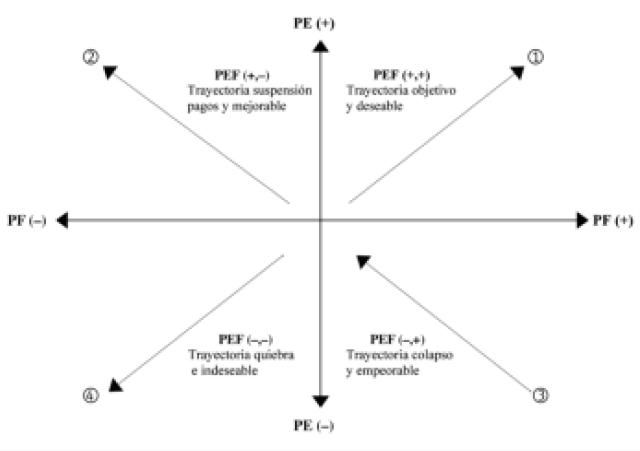
\includegraphics[width = \linewidth]{Imagenes/Las trayectorias economico financieras de la empresa.png}
    \caption{Las trayectorias económico-financieras de le empresa}
    \label{fig:las trayectorias economico financieras de la empresa}
\end{figure}

\subsection{Las zonas del posicionamiento económico financiero}
Un análisis dinámico de la fortaleza económica-financiera de la empresa permitiría, según se observa en la imagen \ref{fig:las trayectorias economico financieras de la empresa}, establecer diferentes trayectorias en la gestión empresarial, y se podrían conceptuar a través de las siguientes, elegidas como más representativas.

\begin{itemize}
    \item La PEF objetivo (+,+). Sin ninguna duda, debería ser la posición ``objetivo'' para cualquier empresa y la que confirmaría el éxito de las funciones directivas integrales. Significaría que la empresa está generando beneficios a través de su actividad económica (PE+) y ademáss presenta una capacidad de pago también positiva (PF+) que la hace rentable y solvente.
    \item La PEF quiebra (-,-). En contra con la anterior, en esta trayectoria tanto la PE como la PF son negativas, situando a la PEF en una posición de total rechazo, de la que hay que salir cuanto antes,d ado el elevado riesgo de colapso y, en términos más jurídicos, de quiebra técnica de la empresa.
    \item La PEF suspensión (+,-). En esta posición, la empresa registra una PE positiva, mientras que la PF es negativa, lo cual quiere decir que la empresa tiene capacidad de producir y vender, y potencialmente retener un beneficio, pero con una PF débil, que la incapacita para atender convenientemente a sus vencimientos de pago. Esta posición es típica de las empresas que registran un crecimiento muy rápido, que tienen éxito pero con crecientes dificultades para conseguir la financiación adecuada, de tal modo que, conforme crece su dimensión y su beneficio, se deteriora su capacidad de afrontar sus compromisos de pago.
    \item La PEF colapso (-,+). En esta posición se registra una PE negativa, cuando la PF es positiva, lo cual quieren decir que la empresa, aunque se encuentra en una posición financiera cómoda y desahogada, sus actividades de explotación no le permiten tener una capacidad de generar beneficios, bien por agotamiento del producto o del mercado, o en el caso contrario, por no haber alzanzado las cuotas de mercados mínimas para convertir la actividad productiva en rentable.
\end{itemize}

\subsection{Las trayectorias desde las posiciones superables}

Contabilidad: recoger, clasificar y resumir los acontecimientos de la vidad de la empresa susceptibles de ser expresados en unidades monetarias.
Limitación significativa: sólo incluye sucesos que pueden cuantificarse de forma objetiva en términos monetarios.

\section{El Plan General de Contabilidad}
\subsection{Marco conceptual}
En los casos de conflicto entre principios contables,d eberá prevalecer el que mejor conduzca a que las cuentas anuales expresen la imagen fiel del patrimonio, de la situación financiera y de los resulados de la empresa.

Principios contables:
\begin{enumerate}
    \item Empresa en funcionamiento. Se considera que el funcionamiento de la empresa tiene una duración ilimitada. ``Los activos para el funcionamiento (terrenos, edificios,...) no se actualizan a valor de mercado, porque su finalidad no es la reventa.''
    \item Devengo. La imputación de ingesos y gastos deberá hacerse en función de la corriente real de bienes y servicios que los mismos representan y con independencia del momento enque se produzca la corriente monetaria o financiera derivada de ellos.
    \item Uniformidad. El criterio adoptado deberá mantenerse en el tiempo.
    \item Prudencia. Únicamente se contabilizarán los beneficios realizadas a la fecha de cierre del ejerciico. Por le contrario, los riesgos previsibles y las perdidas eventuales deberán contabilizarse tan pronto como sean conocidas. ``Los beneficios cuando se realizan, las perdidas cuando se conocen.''
    \item No compensación. En ningún caso podrán compensarse las partidas del activo con el pasivo y propio balance ni la de gastos e ingresos de la cuenta de perdidas y ganancias.
    \item Importancia relativa. Se admitirá la no aplicación estricta de algunos de los principios y critesios contables cuando la importanci arelativa d ela variación que tal hecho produzca no altere la expresión de la imagen fiel.
\end{enumerate}

Los elementos de las cuentas anuales:
\begin{itemize}
    \item Activo: Bienes, derechos y otros recursos controlados económicamente por la empresa, resultantes de sucesos pasados, de los que se espera la empresa obtenga beneficios o rendimientos económicos en el futuro.
    \item Pasivo: Obligaciones actuales surgidas como consecuencia de sucesos pasados, para cuya extinción la empresa espera desprenderse de recursos que puedan producir beneficios o rendimientos económicos en el futuro.
    \item Patrimonio Neto: es la diferencia entre el activo y el pasivo y se identifica con lso recursos propios de los accionistas.
    \item Ingreso: Incrementos en el patrimonio neto de la empresa durante el ejercicio, ya sea en forma de entradas o aumentos en el valor d elos activos, o de disminución de los pasivos, siempre que no tengan su origen en aportaciones, monetarias o no, a los socios o pripietarios.
    \item Gasto: Decrementos en el patrimonio neto de la empresa, ya sea en forma de salidas o fisminuciones en el valor de los activos, o de reconocimiento o aumentos de pasivos, siempre que no tengan la consideración en distribuciones, monetarias o no, a los socios o propietarios.
    \item Cobro: Entrada de dinero en la empresa, cualquiera que sea su origen.
    \item Pago: Salida de dinero de la empresa, cualquiera que sea su destino.
    \item Inversión: Inmovilizaciones de fondos que la empresa no incorpora al proceso productivo (por lo que no se consideran gastos), aunque den lugar a salidas monetarias o compromisos de pago.
\end{itemize}

Reconocimiento de los elementos de las cuentas anuales:
\begin{enumerate}
    \item Que provenga de una transacción de la entidad con otras entidades, de transformaciones internas, así como de otros eventos pasados que la han afectado económicamente.
    \item Satisfacer la definición de un elemento de los estados financieros.
    \item Que sea probable que cualquier beneficio económico asociado con la partida llegue o salga de la empresa, y
    \item Que la partida tenga un coste o valor que pueda ser medido con fiabilidad.
\end{enumerate}

El reconocimiento contable se presenta en dos etapas:
\begin{enumerate}
    \item Reconocimiento inicial. Es el proceso de valuar, presentar y revelar una partida por primera vez en los estados financieros, al considerarse devengada; y
    \item Reconocimiento posterios. Es la modificación de una partida reconocida inicialmente en los estados financieros, originada por eventos posteriores que la afectan de manera particular, para preservar su objetividad.
\end{enumerate}

Valoración de los elemenetos de las cuentas anuales:
\begin{itemize}
    \item Coste histórico
    \item Valor neto realizable o de liquidación
    \item Valor contable o en libros
    \item Valor residual de un activo
    \item Valor razonable o realizable
    \item Valor actual y valor en uso
    \item Coste amortizado
\end{itemize}

Coste histórico de un activo.
Ha sido aplicado tradicionalmente en el modelo contable debido a su fiabilidad porque su determinación y verificación resulta sencilla.
\begin{itemize}
    \item El precio de adquisición de un activo es el importe, en efectivo u otros activos, pagado o pendiente de pago, que corresponda al mismo, así como cualquier coste directamente relacionado con la compra o puesta en condiciones de servicio del activo para el uso al que está destinado.
    \item El coste de producción de un activo incluye el precio de adquisición de las materias primas y otros materiales consumidos, el de los factores de producción directamente imputables al mismo, y la fracción que razonablemente corresponda de los indirectamente relacionados con el activo.
\end{itemize}

Coste histórico de un pasivo.
Es el valor que corresponde a la contrapartida recibida a camnio de incurrir en la deuda o, en algunos casos, la cantidad de efectivo y otros activos líquidos equivalentes que se espere entregar para liquidar una deuda en el curso normal del ejercicio.

Valor contable.
El valor contable de un elemento (ya sea de activo o de pasivo) es el importe neto que está reflejado en la contabilidad de una empresa una vez deducida, en el caso de los activos, la amortización acumulada correspondiente o cualquier corrección de valor del mismo, normalmente por deterioro. Es el valor actualizado del bien, pues se ha tenido en cuenta el paso del tiempo o el uso del mismo. Este valor contable sería el que se debería tener en cuenta a la hora de vender o enajenar el bien.

Valor residual.
Es el valor de la venta del activo tras concluir su vida útil, menos los costes imputables a dicha venta.
\begin{itemize}
    \item Vida útil de un activo es el periodo de tiempo que se espera utilizar el mismo.
    \item Vida económica es el periodo durante el cual se espera que un activo sea utilizable por uno o más usuarios.
\end{itemize}

Valor neto realizable o de liquidación.
Este criterio se aplica, al cierre del ejercicio, cuando la empresa debe evaluar el posible deterioro de las existencias.
\begin{itemize}
    \item Es el importe que la empresa puede obtener por la venta del activo en el mercado, descontando los gastos de la venta.
    \item En el caso de las materias primas y de los productos en curso, los costes estimados serán los necesarios para terminar su producción.
\end{itemize}

Valor razonable.
Este concepto es de uso común en instrumentos financieros: activos y pasivos financieros, combinaciones de negocio y para el cálculo del deterioro.
\begin{itemize}
    \item Es el importe por el que puede ser adquirido un activo o liquidado un pasivo, entre partes interesadas y debidamente informadas, que realizan una transacción en condiciones de independencia mutua.
    \item Si existen mercados activos, la mejor referencia del valor razonable es el precio de cotización.
    \item El valor razonable para los activos para los que no exista un mercado activo se determinará mediante la aplicación de modelos y técnicas de valoración.
    \item Con carácter general los cmabios que tengan lugar en el valor razonable al cierre del ejercicio se reconocerán en la cuenta de pérdidas y ganancias, excepto en algunos casos como los activos financieros disponibles para la venta que los cambios se imputan al patrimonio neto.
\end{itemize}

Valor actual. 
Este criterio se aplica a activos y pasivos que implican, para la emrpesa, el derecho o la obligación de realizar o cobros o pagos.
\begin{itemize}
    \item El valor actual es el importe de los flujos de efectivo futuros esperados actualizados a un tipo de descuento adecuado.
\end{itemize}

Capitalizar.
Si disponemos de una cantidad de dinero $C_0$ al principio del año 1 y la invertimos a un interés anual $r$ en tanto por uno, al final de ese año se habrá convertido en:
\[ C_1 = C_0 (1 + r) \]
y si se vuelve a reinvertir, al final del año segundo será:
\[ C_2 = C_1 (1 + r) = C_0 (1 + r)^2 \]
de la misma manera para $n$ periodos la cantidad será:
\[ C_n = C_0 (1 + r)^n \]

Descontar.
Del mismo modo, a la inversa, si se recibe una cantidad de dinero $C_n$ dentro de $n$ años, su valor actual descontando con la tasa $r$ será:
\[ C_0 = \frac{C_n}{(1 + r)^n} \]

De esta manera podemos representar el valor actual de un conjunto de flujos de caja $C_i$ en sucesivos períodos $i$, dada una tasa de descuento $r$, como:
\[ VA = \sum_{i = 1}^{n} \frac{C_i}{(1 + r)^i} \]


Valo en uso.
Este criterio se aplica al cierre del ejercicio, para determinar si los bienes del inmovilizado material, los intangibles o las inversiones inmobiliarias han sufrido deterioro de valor.
\begin{itemize}
    \item El valor en uso es el importe de los flujos de efectivo futuros esperados actualizados a un tipo de descuento adecuado.
\end{itemize}

Coste amortizado.
El coste amortizado de un activo o pasivo financiero podría entenderse como, el valor actual de los flujos pendientes de cobro o pago, tomando el tipo de interés efectivo de la operación (TIR).

\subsection{Los Estados Financieros}
\begin{itemize}
    \item Balance de situación. Situación de la Compañía en términos financieros a una fecha.
    \item Ceunta de Resultados (P. y G.). Registro de los Ingresos (I) y gastos (G) incurridos por la empresa durante un ejercicio.
    \paragraph{Ingresos.} Son incrementos del patrimonio empresarial, no derivados de aportaciones de socios. Generalmente se derivan de la actividad básica de venta de bienes y prestación de servicios desarrollada por la empresa, sin perjuicio de las condiciones de cobro de la citada venta.
    \paragraph{Gastos.} Son decrementos en el patrimonio empresarial durante el ejercicio por la obtención normalmente de una contraprestación real del exterior, tal como la obtención de bienes o servicios (materias primas, mano de obra, etc.)
    \paragraph{Amortización.} Los bienes de equipo (las inversiones) van perdiendo valor conforme van colaborando en el proceso productivo, incluso por el mero transcurso del tiempo. Se designa por depreciación a esa perdida de valor que experimentan los equipos industrailes o cualquier otro elemento del activo. 
    Al calcular los costes de producción industrial, además de la mano de obra, metrias primas, energía, debemos incluir otros que solo pueden ser expresados de forma indirecta, como la depreciación de las maquinas que se han utilizado para la obtención de los productos. SOn los llamados costes indirectos, donde no existe certeza de imputación a cada producto.
    Denominamos amortización a la imputación de la depreciación al coste de la producción industrial.
    Funciones que cumple la amortización:
    \begin{enumerate}
        \item Función contable: permite reflejar contablemente la perdida de valor de los elementos del activo fijo.
        \item Función económica: a través de la amortización se imputa a los costes de producción un consumo mas, que es el consumo de activo o capital fijo.
        \item Función financiera: Mientras que la capacidad productiva de la empresa se mantiene aproximadamente igual a lo largo de su vida útil, se van acumulando las cuotas de amortización, que la empresa utiliza para hacer frente a sus necesidades financieras.
    \end{enumerate}
    \item Estado de cambios en el Patrimonio Neto
    \item Estado de Flujos de Caja. Clasifica los cobros y pagos en actividades:
    \subitem Operativas (Ingresos y Gastos)
    \subitem De Inversión (Compra y Venta)
    \subitem De Financiación (Inversiones de propietarios y Acreedores)
    \item La Memoria. Completa, amplia y comenta la información contenida en los otros documentos que integran las cuentas anuales. Debe ser información en términos de mínimos:
    \begin{enumerate}
        \item Información narrativa: Debe contener una descripción de la actividad de la compañía, las bases de las cuentas anuales y las normas de valoración aplicadas.
        \item Desglose de numerosas partidas.
        \item Otra información de naturaleza no estrictamente financiera: número de empleados, salarios, dietas...
    \end{enumerate}
\end{itemize}